% This is the Reed College LaTeX thesis template. Most of the work 
% for the document class was done by Sam Noble (SN), as well as this
% template. Later comments etc. by Ben Salzberg (BTS). Additional
% restructuring and APA support by Jess Youngberg (JY).
% Your comments and suggestions are more than welcome; please email
% them to cus@reed.edu
%
% See http://web.reed.edu/cis/help/latex.html for help. There are a 
% great bunch of help pages there, with notes on
% getting started, bibtex, etc. Go there and read it if you're not
% already familiar with LaTeX.
%
% Any line that starts with a percent symbol is a comment. 
% They won't show up in the document, and are useful for notes 
% to yourself and explaining commands. 
% Commenting also removes a line from the document; 
% very handy for troubleshooting problems. -BTS

% As far as I know, this follows the requirements laid out in 
% the 2002-2003 Senior Handbook. Ask a librarian to check the 
% document before binding. -SN

%%
%% Preamble
%%
% \documentclass{<something>} must begin each LaTeX document
\documentclass[12pt,twoside]{reedthesis}
% Packages are extensions to the basic LaTeX functions. Whatever you
% want to typeset, there is probably a package out there for it.
% Chemistry (chemtex), screenplays, you name it.
% Check out CTAN to see: http://www.ctan.org/
%%
\usepackage{graphicx,latexsym} 
\usepackage{amssymb,amsthm,amsmath}
\usepackage{longtable,booktabs,setspace} 
\usepackage{chemarr} %% Useful for one reaction arrow, useless if you're not a chem major
\usepackage[hyphens]{url}
\usepackage{rotating}
\usepackage{natbib}
\usepackage{hhline}
\usepackage{multirow}
\usepackage{adjustbox}
\usepackage{algorithm,algpseudocode}
\usepackage{changepage}

%%% begin alex commands %%%
\newcommand{\Gates}{\text{Gates}}
\newcommand{\InputWires}{\text{InputWires}}
\newcommand{\OutputWires}{\text{OutputWires}}
\newcommand{\Wires}{\text{Wires}}
\newcommand{\Enc}{\operatorname{Enc}}
\newcommand{\Dec}{\operatorname{Dec}}
\newcommand{\compIndist}{\approx_D}
\newcommand{\outputrv}{{\sf output}}
\newcommand{\viewrv}{{\sf view}}

\newcounter{defcounter}
\setcounter{defcounter}{0}
\newenvironment{definition}{\medskip\noindent\refstepcounter{defcounter}{\bf Definition \thedefcounter}\hspace*{2pt}}{\hspace*{\fill}\nopagebreak[4]$\diamondsuit$\medskip}  

\newenvironment{blockquote}{%
  \par%
  \medskip
  \leftskip=4em\rightskip=2em%
  \noindent\ignorespaces}{%
  \par\medskip}

%%% end alex commands %%%



% Comment out the natbib line above and uncomment the following two lines to use the new 
% biblatex-chicago style, for Chicago A. Also make some changes at the end where the 
% bibliography is included. 
%\usepackage{biblatex-chicago}
%\bibliography{thesis}

% \usepackage{times} % other fonts are available like times, bookman, charter, palatino

\title{Two Party Computation}
\author{Alex Ledger}
% The month and year that you submit your FINAL draft TO THE LIBRARY (May or December)
\date{May 2015}
\division{Mathematics and Natural Sciences}
\advisor{Adam Groce}
%If you have two advisors for some reason, you can use the following
%\altadvisor{Your Other Advisor}
%%% Remember to use the correct department!
\department{Mathematics}
% if you're writing a thesis in an interdisciplinary major,
% uncomment the line below and change the text as appropriate.
% check the Senior Handbook if unsure.
%\thedivisionof{The Established Interdisciplinary Committee for}
% if you want the approval page to say "Approved for the Committee",
% uncomment the next line
%\approvedforthe{Committee}

\setlength{\parskip}{0pt}
%%
%% End Preamble
%%
%% The fun begins:
\begin{document}

  \maketitle
  \frontmatter % this stuff will be roman-numbered
  \pagestyle{empty} % this removes page numbers from the frontmatter

% Acknowledgements (Acceptable American spelling) are optional
% So are Acknowledgments (proper English spelling)
    \chapter*{Acknowledgements}
	I want to thank a few people.

% The preface is optional
% To remove it, comment it out or delete it.
\chapter*{Preface}
This is an example of a thesis setup to use the reed thesis document class.



\chapter*{List of Abbreviations}
	You can always change the way your abbreviations are formatted. Play around with it yourself, use tables, or come to CUS if you'd like to change the way it looks. You can also completely remove this chapter if you have no need for a list of abbreviations. Here is an example of what this could look like:

\begin{table}[h]
\centering % You could remove this to move table to the left
\begin{tabular}{ll}
	\textbf{ABC}  	&  American Broadcasting Company \\
	\textbf{CBS}  	&  Columbia Broadcasting System\\
	\textbf{CDC}  	&  Center for Disease Control \\
	\textbf{CIA}  	&  Central Intelligence Agency\\
	\textbf{CLBR} 	&  Center for Life Beyond Reed\\
	\textbf{CUS}  	&  Computer User Services\\
	\textbf{FBI}  	&  Federal Bureau of Investigation\\
	\textbf{NBC}  	&  National Broadcasting Corporation\\
\end{tabular}
\end{table}
	

    \tableofcontents
% if you want a list of tables, optional
    \listoftables
% if you want a list of figures, also optional
    \listoffigures

% The abstract is not required if you're writing a creative thesis (but aren't they all?)
% If your abstract is longer than a page, there may be a formatting issue.
    \chapter*{Abstract}
	The preface pretty much says it all.
	
	\chapter*{Dedication}
	You can have a dedication here if you wish.

  \mainmatter % here the regular arabic numbering starts
  \pagestyle{fancyplain} % turns page numbering back on

%The \introduction command is provided as a convenience.
%if you want special chapter formatting, you'll probably want to avoid using it altogether

\chapter*{Introduction}
     \addcontentsline{toc}{chapter}{Introduction}
\chaptermark{Introduction}
\markboth{Introduction}{Introduction}
% \onehalfspacing
% \doublespacing

 Introduction goes here

\chapter{Background}

Multiparty computation (MPC) is the study and creation of protocols for computing a function between multiple parties, such that no party learns the input of any other party.

The idea is best communicated through an example: suppose Alice and Bob are millionaires and wish to determine who is wealthier, but Alice and Bob are also secretive, and do not want to disclose their exact amount of wealth. 
Is there some method by which they can determine who has more money?

The goal of MPC is to design a protocol which will help Alice and Bob solve their problem.
The desired properties of a secure MPC scheme can be informally described as follows:
\begin{itemize}
    \item \textbf{Privacy:} Each party's input is kept secret.
    \item \textbf{Correctness:} The correct answer to the computation is computed.
\end{itemize}

Originally, the goal was to come up with a protocol that was secure and prove that the protocol was secure. 
In more recent times, the focus has shifted to making the MPC faster, fast enough that it can be used regularly in the real world.

If MPC can be made fast enough, it could serve a wide range of applications.
For example, imagine that two companies who operate in a similar industry want to work together, but they don't want to disclose any company research which the other doesn't know.
These companies could a run set intersection function (a function that given two inputs finds their intersection, or overlap), to determine what information they can disclose without giving away important information.

Another interesting example of MPC is to improve the outsourcing of computation.
As it is right now, cloud computing companies, such as Amazon and Google, have really nice computers which they will rent out to you. 
You can pay them someone money, write a program, and run it on their computers. 
The problem is that you may not trust the cloud computing company, and you want some guarantees that they are going to respect the privacy of your computation.
An MPC protocol, in this setting, would allow you to run computation in the cloud, with the guarantee that the inputs to your computation are disguised.

Since the research into MPC has focused on creating a method by which an arbitrary function can be computed securely, the application of MPC beyond what we can presently conceive of. 
It's not unlikely that MPC protocols will become a standard in the internet, where when you access the internet, behind the scenes your access is being is plugged into an MPC protocol, sent off to another computer to do some processing. 
As cryptography improves, research in MPC and other areas of cryptography, the hope is that the security of our computer systems will improve as well.
However, there is no guarantee. 
The modern cryptography needs to implemented and used, perhaps in some cases built into low-level standards, and used correctly.
At this point, the outlook of cryptography is bright, but the future will only be realized positvely if it is actively worked towards.

\section{Tools for MPC}
Imagine again that millionaires Alice and Bob wish to determine who has more wealth.
Suppose that Alice has $x_a$ dollars and Bob has $y_b$ dollars.
Then the function that they wish to compute is $f: \{0,1\}^n \to \{0,1\}$ as defined by:
\begin{equation}
    \label{eqn:less_than}
    f(x_a,x_b) = 
    \begin{cases}
    0, & x_a \leq x_b; \\
    1, & \text{otherwise}.
    \end{cases}
\end{equation}

\textbf{Why is this here?}
If Alice and Bob successfully compute $f(x,y)$ and each gets the output, then each party has gained some knowledge about the nature of the other's input.
For example, if $f(x_a,x_b)$ outputs $0$, then Alice and Bob know that Alice has more money.
Alice has learned that Bob has less than $x$ dollars, and Bob has learned that Alice has more $x_b$ dollars.
Therefore it's not possible for MPC to guarantee that \textit{no} information about the other parties' inputs is learned, only that nothing more is learned than what can be inferred from a single party's input and the output of $f$. 

MPC requires a combination of several cryptographic tools.
The next few sections will describe these basic tools, and then MPC will described in section $x$. 
tools discussed are 
\begin{enumerate}
    \item Boolean Circuit
    \item Encryption
    \item Oblivious Transfer (need to explain semihonest and honest)
\end{enumerate}

\subsection{Encryption}
Encyprtion is the process of encoding a message such that only parties with the key can read the message.
An encryption protocol is composed of two parts.
The first part is the encryption function which disguises the message, and the second part is the decryption function which unobfuscates the disguised message.
We notate encryption and decryption with
\begin{equation}
    \label{eqn:encryption}
    \begin{split}
        \Enc_k (pt) & = ct  \\
        \Dec_k(ct) & = pt
    \end{split}
\end{equation}
where $pt$ stands for plaintext and is the original message, $ct$ stands for ciphertext and is the encrypted message, $k$ is the secret key, that only authorized readers of the message hold, and is a random sequence of $\lambda$ $0$s and $1$s, and $\lambda$ is a security parameter of our protocol (As $\lambda$ increases, the size of the key increases, and so the encryption becomes harder to break.)

The encryption decribed above is more precisely called symmetric-key encryption, as opposed to public-key encryption.
The difference between the two is that for symmetric-key encryption, there is a single key and all communicating must have the same key in order to acheive secure communication, whereas in public-key encryption, the encryption key is published publicly, and anyone can send a message using the public key, and the message can only be decrypted by those with the secret key.
For more information on encryption, we encourage the reader to peruse the many great online resources.

The MPC protocols that will be examined here exclusively use symmetric-key encryption.

\subsection{Digital Signatures/MACS}
kA
Do we need this?

\subsection{Boolean Circuit} 
A function for an MPC protocol is represented by a boolean circuit.
A boolean circuit takes as input a sequence of $n$ $0$s and $1$s, (i.e. a value in $\{0,1\}^n$), performs a series of small opreations on the inputs, and outputs a sequence of m $0$s and $1$s (i.e. a value in $\{0,1,\}$).
You may have encountered circuits and logical operators in another context, where the inputs and outputs were True and False.
For our usage, True will correspond to the value $1$, and False will corresond to the value $0$. 

The small operations performed inside of a circuit are performem by an object called a \emph{gate}.
A gate is composed of three wires: two input wires and one output wire, where a \emph{wire} can have a value either $0$ or $1$.
A gate performs a simpler operation on the two inputs, resulting in a single output bit.
Table \ref{tab:xor} gives the mapping of an XOR gate.

\begin{table}[h]
\label{tab:xor}
\centering
\begin{tabular}{ | l | c || r |}
\hline
x & y & xor(x,y) \\ \hline
1 & 1 & 0 \\ \hline
1 & 0 & 1 \\ \hline
0 & 1 & 1 \\ \hline
0 & 0 & 0 \\ \hline
\end{tabular}
\caption{The mapping of an XOR gate.}
\end{table}

A circuit is a combination of gates. 
In fact, a circuit built out of only AND gates, XOR gates and NOT gates can compute any function.
\textbf{Find details and citation} In other words, if there's some algorithm that do it, then there is some circuit that can do it as well.
Hence, a circuit is a sufficient representation of the function $f$.
Figure \ref{fig:less_than_circuit} shows the circuit representation of a circuit that computes the less than function, the function $f$, specified in equation \ref{eqn:less_than} that millionaires Alice and Bob wanted to compute.

\begin{figure}[h]
    \centering
    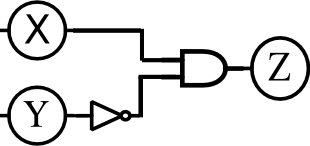
\includegraphics[scale=0.75]{images/drawing.png}
    \label{fig:less_than_circuit}
    \caption{A circuit that computes the less or equal to function, equivalent to $f$ for input of two one-bit values. \textbf{TODO, add truth table?}}
\end{figure}

A circuit \textbf{with what constraints???} can compute any function.

\subsection{Technical Definition of a Circuit}
A circuit, which I will refer to as $g$, is formalized by a 6-tuple $g = (n,m,q,A,B,G)$, where $n$ is the number of inputs, $m$ is the number of outputs and $q$ is the number of gates.
We define $r = n + q$ to the number of wires inside of the circuit.
We let $\Wires = \{1,\ldots, n+q\}, \InputWires = \{1,\ldots, n\}, \OutputWires = \{n+1-m+1, \ldots,n+q\}$, and $\Gates = \{n+1, \ldots, n+q\}$.
Then $A : \Gates \to \Wires \setminus \OutputWires$ identifies each gate's first incoming wire.
And $B : \Gates \to \Wires \setminus \OutputWires$ identifies each gate's second incoming wire.
Finally, $G: \Gates \times \{0,1\}^2 \to \{0,1\}$ identifies the functionality of each gate.

For example, the less than circuit shown in figure \ref{fig:less_than_circuit} has values:

<<<<<<< HEAD
\newcommand{\Gb}{\operatorname{Gb}}
\newcommand{\En}{\operatorname{En}}
\newcommand{\De}{\operatorname{De}}
\newcommand{\Ev}{\operatorname{Ev}}
\newcommand{\ev}{\operatorname{ev}}
\newcommand{\evcirc}{\ev_{circ}}

\newcommand{\fbar}{f^-}
\newcommand{\Topo}{\operatorname{Topo}}
\renewcommand{\algorithmicrequire}{\textbf{Input:}}
\renewcommand{\algorithmicensure}{\textbf{Output:}}

To evaluate a circuit, we use a canonical algorithm $\evcirc$.
$\evcirc$ takes as input a string $f$ and a string $x = x_1 x_2 \ldots x_n$ and does the following:

\begin{algorithm}
\caption{$\evcirc$}
\label{alg:evcirc}
\begin{algorithmic}
\Require Function $f$ and String $x = x_1, \ldots x_n$.
\Ensure Output of function $f$ on input $x$.
\State $(n,m,a,A,B,G) \gets f$
\Comment parse $f$ as a circuit
\For{$g = n+1$ to $n+q$} 
\Comment loop over all gates.
\State $a \gets A(g)$
\Comment compute each gate
\State $b \gets B(g)$
\State $x_g \gets G_g(x_a, x_b)$
\EndFor \\
\Return $x_{n+q-m+1} \ldots x_{n+q}$
\end{algorithmic}
\end{algorithm}

\begin{definition}{Topological Circuit}
    A topological circuit, denoted $\fbar$, is the $5$-tuple $(n,m,q,A,B)$ for some circuit $f = (n,m,q,A,B,G)$.
    Furthermore, define $\Topo(f)$ such that $\fbar = \Topo(f)$.
\end{definition}

A topological circuit is the same as its conventional circuit $f$, except that the functionality of the gates is not specified.
If one holds a topological circuit, then they know the structure of the function, but not what is being computed.
=======
\subsection{Encryption}
Encryption is a method of encoding a message such that only parties with the key can read the message.
An encryption protocol is composed of two parts.
The first part is the encryption function which disguises the message, and the second part is the decryption function which unobfuscates the disguised message.
We notate encryption and decryption with
\begin{equation}
    \label{eqn:encryption}
    \begin{split}
        \Enc_k (pt) & = ct  \\
        \Dec_k(ct) & = pt
    \end{split}
\end{equation}
where $pt$ stands for plaintext and is the original message, $ct$ stands for ciphertext and is the encrypted message, $k$ is the secret key, that only authorized readers of the message hold, and is a random sequence of $\lambda$ $0$s and $1$s, and $\lambda$ is a security parameter of our protocol (As $\lambda$ increases, the size of the key increases, and so the encryption becomes harder to break.)

The encryption decribed above is more precisely called symmetric-key encryption, as opposed to public-key encryption.
The difference between the two is that for symmetric-key encryption, there is a single key and all communicating must have the same key in order to acheive secure communication, whereas in public-key encryption, the encryption key is published publicly, and anyone can send a message using the public key, and the message can only be decrypted by those with the secret key.
For more information on encryption, we encourage the reader to peruse the many great online resources.

The MPC protocols that will be examined here exclusively use symmetric-key encryption.

\subsection{Digital Signatures/MACS}
Do we need this?

\subsection{The DDH Assumption} \label{sctn:DDH}
When a cryptographic scehe is said to be \textit{secure}, cryptographers actually mean something much more precise. 
When a cryptographic scheme is considered secure, it actually means that an adversary can beat the scheme only if the adversary can tackle the hardness assumptions on which the scheme is based.
A common hardness assumption in crytoraphy is the Decisional Diffie-Helman Assumption (DDH Assumption), an assumption about solving a problem concerning discrete logs.

Informally, the DDH assumption is:
\begin{equation}
	\label{eqn:DDH}
	\begin{split}
	& \qquad \text{Let $G$ be a group of order $q$ with generator $g$.} \\
	& \qquad \text{Let $a, b$ and $c$ be random elements from $\mathbb{Z}_q$.} \\
	& \qquad \text{Then, $(g^a, g^b, g^{ab}) \compIndist (g^a, g^b, b^c)$}. 
	\end{split}
\end{equation}

\textbf{Define computationally indistinguishability somewhere}

\subsection{Oblivious Transfer}
Oblivious Transfer is a special method of communicating a message between two parties where a sender sends one of two messages the receive, and the sender remains oblivious as which message was sent.
The setup is the following:
Alice has two messages, $m_1$ and $m_2$, and he wants to send a message to Bob under the following conditions: First, Alice sends either $m_1$ or $m_2$ but not both. Second, Alice does not know which message he sent to Bob. Third, Bob selects which message he wants to receive.

Here we give the Naor-Pinkas protocol of $1-2$ oblivious transfer.
The protocol relies on the DDH assumption (see section \ref{sctn:DDH}) and is secure in the semi-honest setting (see section \ref{sctn:semihonest}).

\begin{figure}
    \centering
    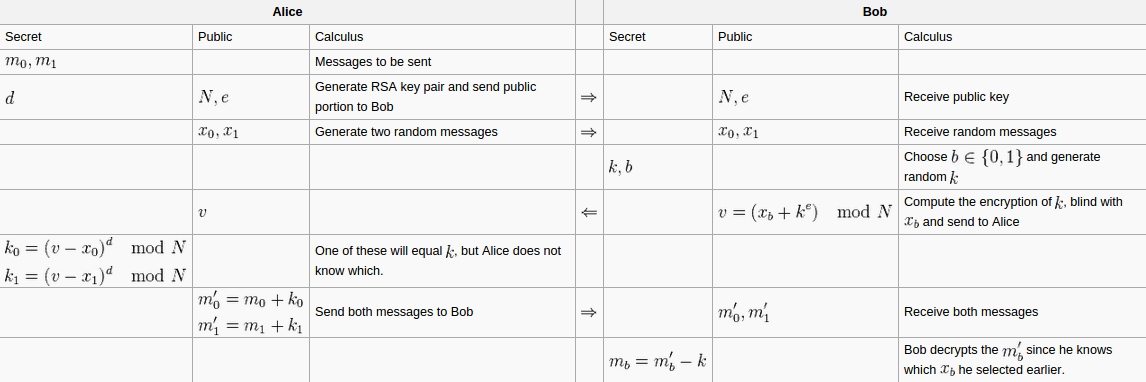
\includegraphics[scale=0.3]{images/ot_wiki}
    \caption{Semi-honest Naor-Pinkas oblivious transfer.}
\end{figure}

Researchers have also developed methods for performing k-out-of-n oblivious transfer, where the sender sends exactly $k$ messages out of a possible $n$.
The method described above is called $1-2$ oblivious transfer, and is the OT used in MPC protocols.

Since the first proposal of OT in \textbf{year}, several improvements have been developed.
Preprocessing.
OT extension.
Semi-honest/Malicious.

\subsection{Other}
\textbf{TODO}
Paper has topological circuit next to real circuit
change arbitrary function to arbitrary boolean function.

\section{Classic MPC}
MPC was first proposed by Andrew Yao in an oral presentation on secure function evaluation.
After Yao's presentation, two methods for performing MPC were developed.
One method was contributed by Yao himself, and the other was contributed by a group of researchers, Beaver, Micali and Widgerson.
The two methods are premised on a similar idea: encrypt a circuit by encrypting its gates, with has since been termed garbled circuit.
At this point, it is unclear which method is better, both in terms of security and in terms of speed speed. 
As a result, research is still being done on both protocols.

This section will first give a new definition of a garbling scheme, first presented by BHR in 2012, and then give Yao's garbled circuit protocol, and finally GMW's garbled circuit protocol.

\subsection{Garbling Schemes}
Recall millionaires Alice and Bob who want to determine who has more wealth.
Alice and Bob start with a function $f$ (defined in \ref{function}) and their inputs, $x_a$ and $x_b$, which correspond to their amount of wealth.
In order to compute who has more money, the function $f$ needs to be transformed such that they can compute the function by sending messages between each other their inputs, $x_a$ and $x_b$, which correspond to their amount of wealth.
Informally, a garbling scheme transforms a specification of a function into a collection of algorithms which can in combination can compute the function.

\begin{definition}{Garbling Scheme}
    A garblering scheme is a $5$ tuple of algorithms $G = (\Gb, \En, \De, \Ev, \ev)$ where the algorithms are
    \begin{itemize}
        \item $\Gb(f, k) \rightarrow (F,e,d)$. 
        \item $\En(e,x) \rightarrow X$.
        \item $\Ev(F,X) \rightarrow Y$.
        \item $\De(d,Y) \rightarrow y$.
        \item $\ev(f, x) \rightarrow y$.
        where 
        \begin{itemize}
            \item $f$ is a function.
            \item $k \in \mathbb{N}$ is the security parameter.
            \item $x \in \{0,1\}^n$ is the initial input.
            \item $X$ is the garbled input
            \item $Y$ is the garbled output
            \item $y$ is the final output
            \item $F$ is a string that describes the operation of the $\Ev$ algorithm. 
            \item $e$ is a string describing the operation of the $\En$ algorithm. In particular, $e$ describes how to obscure the input $x$.
            \item $d$ is a string describing the operation of the $\De$ algorithm. In particular, $d$ describes how to unobscure the output $Y$.

        \end{itemize}
        \item A garbling scheme guarantees correctness if $\De(d, \Ev(F, \En(e,x))) = \ev(f,x)$.
    \end{itemize}
    A garbling schemes map the information:
\begin{equation}
    (f,k,x) \rightarrow^{\Gb} (F,e,d,x) \rightarrow^{\En} (F,d,X) \rightarrow^{\Ev} (d,Y) \rightarrow^{\De} y
\end{equation}
\end{definition}

To make the idea a garbling scheme more concrete, below is an example of how Alice and Bob would compute who is wealthier. 
The inputs to their computation are $f$, the function to be computed which is defined in equation \ref{eqn:less_than}, and their inputs $x_a$ and $x_b$.
\begin{enumerate}
    \item Alice has the function $f$ to be computed, her input $x_a$, and Bob has his input $x_b$.
    \item Alice hard-codes her inputs into the function, resulting in $\hat{f}$.
    \item Alice runs the probabilistic algorithm $\Gb(\hat{f}, k)$. She now has $(F,e,d)$.
    \item Alice encodes all possible inputs that Bob could, all possible sequences of $0$s and $1$s, into $X$ using $\En$.
    \item Alice sends $(F,X,d)$ to Bob.
    \item Bob runs $\Ev(F,X)$ to get $Y$. This computes the function, but the output, $Y$, is obscured.
    \item Bob runs $\De(d,Y)$ to get $y$. This unobscures the output $Y$. Bob now has $y \in \{0,1\}$.
        If $y = 0$, then Bob knows that Alice is wealthier. 
        If $y = 1$, then Bob knows that he is wealthier.
    \item Bob sends $y$ to Alice.
\end{enumerate}

The definition of a garbling scheme is a recently created definition, proposed for the first time ****, *** years after Yao's garbled circuit was proposed.
The benefits of thinking of a garbled scheme in terms of this definition are significant.
For one, it easier to map a theoretically garbling protocol into practice, i.e program it. 
The methods are already separated, whereas before the algorithm was generally one giant idea.
When the methods are separated, the programmer does not need to intimately understand the security guarantees and pitfalls of the method, as the sequence of events that need to happen is explicit in the construction.
A second reason that this definition of a garbling scheme is good is that it presents garbling as a larger cryptographic abstraction. 
Garbling schemes are simply methods for garbling a function and input, and this definition matches the intuition. 

\subsection{Projective Garbling Schemes}
Perhaps a helpful abstraction to have later.

\subsection{Security of Garbling Schemes}
This section will give the definition of security of a garbling scheme.

\subsection{MPC Security Definitions}
A number of definitions which formalize what it means for a multiparty computation have been formalized. 
Yao, in his 1982 paper on secure function evaluation, says a 2PC protocol is secure if it has the property:

\begin{blockquote}
If one participant behaves according the the protocol, the probability that the other participant successfully cheats is at most $\gamma$ for $\gamma \in \{0,1\}$.
\end{blockquote}

Since Yao's original definition, many other definitions for the security of 2PC protocols have been proposed.
Here we give Goldreich's definition of 2PC, which is given in his textbook \textit{Foundations of Cryptography Volume II}, and is reproduced in various papers, most notably Lindell and Pinkas 2009 survey paper on multiparty computation \cite{goldreich2, lindell2009}.

%As more complex protocols were developed, both for MPC, and in other areas of cryptography, property based definitions became difficult to work with.
%The main problem that it was unclear precisely what assumptions were being made about what each party could and couldn't do. 
%For example, in Yao's definition above, it's not clear that the parties' inputs are kept secret if both parties behave according to the protocol.
%At the least, the definition doesn't give any guarantee.
%For a while, cryptographers added in additional properties to definitions, but eventually it became clear that there was always the possibility that a certain property was being missed.

%This led to the creation to indistinguishability and simulation based definitions of security.
%The idea is that the adversary cannot tell what is going on, based on the information that they receive, so the best that the adversary can possible do is guess what is happening.
%For example, a definition of a secure encryption scheme could be:
%\textbf{Might give the definition of encryption in the section above. If we do, just reference that section. That might be preferable}

%\begin{blockquote}
%\begin{itemize}
%	\item Adversary picks two messages, $m_0$ and $m_1$. 
%	\item We pick a random bit $b \in \{0,1\}$. Encrypt $m_b$, and send the encrypted version to the adversary (i.e. send $c = \Enc(m_b)$).
%	\item Adversary outputs a bit $b'$ where $b' = 0$ if they believe the encrypted messages was $m_0$, and $b' = 1$ if they think the encrypted message was $m_1$. 
%	\item Finally, we consider the encryption scheme secure if
%	$$Pr[\text{Adversary outputs $b' = b$}] \approx_C \frac{1}{2}.$$
%\end{itemize}
%\end{blockquote}
%
%The cryptography research community now tends to prefer simulation based definitions. 
%The idea behind simulation based definitions is that we have ideal world, in which the protocol is run perfectly and securely, and then we have the real world protocol, the one that Alice and Bob run. 
%Then, for some adversary, we randomly choose either the real ideal or real world and run the MPC computation with the adversary in that world.
%The adversaries attempts to determine which world the protocol is being run in.
%Finally, the protocol is secure if the adversary can't do any better than guessing which world they are in.
%As a consequence, the real world is indistinguishable from the ideal world, hence cryptographers feel confident that the protocol is secure. 
%The idea being that if the adversary could learn more information in the real world, say information about other parties' inputs, then they would know that they are in the real world, hence the protocol is insecure. 
%
%The biggest problem with simulation based definitions is that it is difficult and labor intensive to prove with the definition.
%The property based definitions are the most straightforward to prove, and the most familiar to proofs used in mathematics.
%

\subsection{Goldreich and Lindell's Definition of Security for 2PC}
%The definition is designed for static, semi-honest adversaries. 

\begin{description}
\item [Setup:] \hfill
    \begin{itemize}
        \item Let $f = (f_1, f_2)$ be a probabilistic, polynomial time functionality. 

        \item Let $\Pi$ be a two party protocol for computing $f$. 

        \item Define $\viewrv_i^{\Pi}(n,x,y)$ (for $i \in \{1,2\}$) as the view of the $i$th party on input $(x,y)$ and security parameter $n$.
        $\viewrv_i^{\Pi}(n,x,y)$ equals the tuple $(1^n, x, r^i, m_1^i, \ldots, m_t^i)$, where $r^i$ is the contents of the $i$th party's internal random tape, and $m_j^i$ is the $j$th message that the $i$th party received.
    
        \item Define $output^{\Pi}_i(n,x,y)$ as the output of the $i$th party on input $(x,y)$ and security parameter $n$.
        Also denote
        $$ \outputrv^{\Pi}(n,x,y) = (\outputrv^{\Pi}_1(n,x,y), \outputrv^{\Pi}_2(n,x,y)).$$

    \item Note that $\viewrv^{\Pi}_i$ and $\outputrv^{\Pi}_i$ are random variables whose probabilities are taken over the random tapes of the two parties. Also note that for two party computation.
\end{itemize}
\item [Definition:]
We say that $\Pi$ securely computes $f$ in the presence of static semi-honest adversaries if there exists probabilistic polynomial time algorithms $S_1$ and $S_2$ such that for all $x,y \in \{0,1\}^*$, where $|x| = |y|$, the following are true:
\begin{equation} 
    \label{eqn:secdef1}
    \{(S_1(x, f_1(x,y), f(x,y)))\}_{x,y} \equiv^C \{(\viewrv^{\Pi}_1(x,y), \outputrv^{\Pi}(x,y)) \}_{x,y} 
\end{equation}
\begin{equation} 
    \label{eqn:secdef2}
    \{(S_2(x, f_2(x,y), f(x,y)))\}_{x,y} \equiv^C \{(\viewrv^{\Pi}_2(x,y), \outputrv^{\Pi}(x,y)) \}_{x,y} 
\end{equation}

\item[Intuition:]
    We think of $\viewrv^{\Pi}_i$ as all of the information that the $i$th has to operate with, such that any conclusion that the $i$th party can come to could be determined from $view^{\Pi}_i$.
    Moreover, $\outputrv^{\Pi}_i$ is simply a complicated way of writing the output of the $i$th party. 
    The value of $\outputrv^{\Pi}_i$ is computable from the tuple $\viewrv^{\Pi}_i$.

    Let's dig a little deeper into the meanings of equation \ref{eqn:secdef1} and \ref{eqn:secdef2}.
    They state that a probabilistic, polynomial time algorithm, denoted $S_1$ and $S_2$, which is given access \textit{only} to the party's input and output can compute the view of a party.
    For example, the definition requires that $S_1$ on input $(x, f(x,y))$ must be able to compute $\viewrv^{\Pi}_i(x,y)$, in particular the messages received by party 1, such that the generated view is indistinguishable from the actual view.
If there exists an algorithm that can perform the aforementioned task, then $\Pi$ does not adequately conceal information, so we should not consider $\Pi$ to be secure.

    Finally, the definition requires that $|x| = |y|$; however, this constraint can be overcome in practice by padding the shorter input.
\end{description}

The definition of security provided here only applies when adversaries are semi-honest (see \ref{semihonest section}).
Definitions of security in settings with malicious adversaries require substantially more complexity.
As a result, these definitions are often simulation based definitions.
They imagine an ideal world, where the function $f$ must be computed securely, and by a series of comparisons, show that the real world where $\Pi$ computes $f$ is essentially the same as the ideal world.
For an easy to understand security definition of 2PC with malicious adversaries, we refer to reader to \cite{lindell2009}.

\subsection{Yao's Garbled Circuit}
We now give an implementation of a generic 2PC protocol created by Yao \cite{yao}.
The protocol works for two parties; we will call party 1 Alice, denoted $A$, and party 2 Bob, denoted $B$, who have inputs $x$ and $y$ respectively.
Suppose $f$ is the function that Alice and Bob wish to compute.

Yao's protocol depends on first encoding the function $f$ as a circuit, as discussed in more detail in section \ref{sctn:circuits}, and then Alice and Bob together evaluate the circuit.

% (complexity - add to end) The number of round is constant.
% 1 OT per input wire of party B + enc/dec for each gate.

\begin{algorithm}
\caption{Garble Circuit}
\label{alg:garble}
\begin{algorithmic}
    \Require Circuit $f(x,\cdot)$ 
    \Ensure Populate garbled tables $f(x,\cdot).tables$.
\For{wire $w_i$ in $f(x,\cdot).wires$} 
    \State Generate two encryption keys, called garbled values, $W_i^0$ and $W_i^1$.
    \State Assign $(W_i^0, W_i^1)$ to $w_i$.
\EndFor \\

\For{gate $g$ in $f(x,\cdot).gates$}
    \State Let $w_i$ be $g$'s first input wire.
    \State Let $w_j$ be $g$'s second input wire.
    \State Let $w_k$ be $g$'s output wire.
    \For{$(u,v) \in \{(0,0), (0,1), (1,0), (1,1)\}$}
    \State $T_g[u,v] = \Enc_{W_i^u}( \Enc_{W_j^v} ( W_k^{g(u,v)}))$
    \EndFor
    \State $f(x,\cdot).tables[g] = T_g$.
\EndFor
\end{algorithmic}
\end{algorithm}

\begin{algorithm}
\caption{Evaluate Circuit}
\label{alg:evaluate}
\begin{algorithmic}

\Require $(input\_wires, tables, gates)$
\For{Input wire $w_i$ in $input\_wires$}
	\Comment retrieve garbled values of input wires
	\State Perform OT$(w_i, x_i)$ 
	\Comment retrieve $W^{x_i}_i$ from Alice
	\State Save the value to $w_i$.
\EndFor

\For{Gate $g$ in $gates$}
	\Comment compute the output of each gate.
	\State Let $w_i$ be $g$'s first input wire.
	\State Let $w_j$ be $g$'s second input wire.
	\State Let $w_k$ be $g$'s output wire.
	\State \textbf{Require} $w_i$ and $w_j$ have been assigned garbled values.
	\State \textbf{Require} $w_k$ has not been assigned a garbled value.
    	\For{$(u,v) \in \{(0,0), (0,1), (1,0), (1,1)\}$}
		\State $temp = \Dec_{w_j}(\Dec_{w_i}(tables[g][u,v]))$
		\If{$temp$ decrypted correctly}
			\State $w_k = temp$
		\EndIf
	\EndFor
\EndFor
\end{algorithmic}
\end{algorithm}

\subsubsection{Step 0: Setup}
Alice and Bob want to compute the function $f(x,y)$, where $x,y \in \{0,1\}^*$.
Alice is the garbler, and will create the circuit.
Bob is the evaluator, and will compute the circuit.
Alice first hardwires her inputs into the circuit, yielding a circuit that computes $f(x,\cdot)$.

\subsubsection{Step 1: Garbling the Circuit}
Alice garbles each gate, according to the algorithm outlined in Algorithm \ref{lag:garble}, which produces a table $T_g$ for each gate $g$.
The table enables the computation of $g$, if one is given either $W^0_i$ or $W^1_i$ and either $W^0_j$ or $W^1_j$ where wire $i$ and $j$ are the input wires to $g$.
Figure \ref{example} gives an example of a table for an AND gate. \textbf{TODO}

\subsubsection{Step 2: Bob's Input and Computing the Circuit}
Alice sends the garbled circuit to bob, which consists of the garbled tables, $f(x,\cdot).tables$, and the rules for connecting the gates together.
In order for Bob to compute the circuit, he needs the garbled values of all input wires.
Once he has the garbled values of the input wires, he can decrypt the first few gates, and acquire the decryption keys of the other gates until he has the keys to decrypt all of the gates in the circuit, yielding the output.
Bob can acquire the garbled values of the input wires from Alice using 1-out-of-2 oblivious transfer on each input wire (see section \ref{sctn:oblivious_transfer}).
If necessary, Bob sends the final output of the circuit to Alice. 
This is necessary only if $f_1(x,y) = f_2(x,y)$. 
Bob's protocol is outlined in more detail in Algorithm \ref{alg:evaluate}.

\subsubsection{Explanation of the security of Yao's protocol}
To do.

\subsubsection{Notes about complexity}
1 OT per (input?) wire.
How much encryption?
Not good enough for practice.

\subsection{GMW}
Where Yao's protocol is premised on encrypting gates individually, GMW's protocol for garbling circuits is premised on secret sharing, and performing operations on the shared secrets. 
Secret sharing, in its general idea, is class of methods for distributing a secret to a group of participants, where each participants is allocated a \textit{share} of the secret. 
The secret can only be reconstructed when a sufficient number of the participants combine their shares, but any pool of insufficient shares yields no information about the secret.

GMW begins by having Alice and Bob secret share their inputs, so each party now has a collection of \textit{shares}. 
Algorithm \ref{alg:gmw_setup} describes this process in more detail.
Then Alice and Bob perform a series of operations on their shares, which are dictated by the gates in the function they wish to compute.
As with Yao's protocol, a gate may either compute XOR, AND or NOT.
Each operation requires a different series of operations, which are described in Algorithm \ref{alg:gmw_gates}.
Finally, Alice and Bob publicize their shares to each other, at which point each party will have sufficient shares to compute the output of the function.

\begin{algorithm}[h!]
\caption{GMW Setup}
\label{alg:gmw_setup}
\begin{algorithmic}
% http://crypto.biu.ac.il/gmw-multi-party-protocol-and-oblivious-transfer-extension
    \State Alice does the following on input Circuit $f(x,\cdot)$ and $x = x_0x_1\ldots x_n$
    \For{wire $w_i$ in $f(x, \cdot).wires$}
        \State Assign $a^1_{w_i} \leftarrow \{0,1\}$
        \Comment a uniform random selection of $0$ or $1$.
        \State Assign $b^1_{w_i} = x_i \oplus a_{w_i}^1$
    \EndFor
    \State Bob does likewise on input Circuit $f(x,\cdot)$ and $y = y_0y_1\ldots y_n$
    \State Hence Alice has generated shares $\{a^1_w, b^1_w\}_w$ 
    \State and Bob has generated shares $\{a^2_w, b^2_w\}_w$
    \State Alice and Bob divide the shares such that Alice has all $a_w$ and Bob has all $b_w$.
\end{algorithmic}
\end{algorithm}

\begin{algorithm}
\caption{GMW Gate Evaluation}
\label{alg:gmw_gates}
\begin{algorithmic}
    \State \textbf{XOR Gate}
    \Comment $x_i \oplus y_i = (a_{w_i}^1 \oplus b_{w_i}^1) \oplus (a_{w_i}^2 \oplus a_{w_i}^2)$
    \State Alice evaluates $a_{w_i}^1 \oplus a_{w_i}^2$
    \State Bob evaluates $b_{w_i}^1 \oplus b_{w_i}^2$
    \\
    
    \State \textbf{AND Gate}
    \Comment $x_i \wedge y_i = (a_{w_i}^1 \oplus b_{w_i}^1) \wedge (a_{w_i}^2 \oplus a_{w_i}^2)$
    \State Alice samples $\sigma \leftarrow \{0,1\}$
    \Comment a uniform random selection of $0$ or $1$
    \State Alice constructs table $T$:
     \For{$(u,v) \in \{(0,0), (0,1), (1,0), (1,1)\}$}
     	\State $T[u,v] = (a^1_{w_i} \oplus u) \wedge (a^2_{w_i} \oplus v)$
	\State $s[u,v] = \sigma \oplus T[u,v]$.
     \EndFor    
     \State Do 1-4OT. Alice sends $(s[0,0], s[0,1], s[1,0], s[1,1])$ 
     \State Bob selects result based on $(u,v) = (b^1_{w_i}, b^2_{w_i})$.
    \\
    
    \State \textbf{NOT Gate}
    \Comment $w_i = (\neg a_{w_i}) \oplus (\neg b_{w_i})$
    \State $\triangleright$ Evaluate the negative of a particular wire $w_i$. 
    \State $w_i = a_{w_i} \oplus b_{w_i}$
    \State Let $a'_{w_i} = 1 \oplus a_{w_i}$
    \Comment i.e. $a'_{w_i} = \neg a_{w_i}$
    \State Let $b'_{w_i} = 1 \oplus b_{w_i}$
    \Comment i.e. $b'_{w_i} = \neg b_{w_i}$
    
    
    
\end{algorithmic}
\end{algorithm}


\section{Improving MPC}
\subsection{Overview of history}
working on specific function verse general functions
working on number of parties
making it work for sugarbeet auction
election potential?
auctions


\subsection{Point and Permute}
\subsection{Garbled Row Reduction 3}
\subsection{Free XOR}
\subsection{Garbled Row Reduction 2}
\subsection{FlexXOR}
\subsection{Half Gates}

\section{Overview of what's going to be covered}

\begin{table}[h]
  \centering
  \renewcommand{\arraystretch}{1.2}
\begin{adjustbox}{width=1\textwidth}
  \begin{tabular}{|p{5cm}||c|c||c|c||c|c||c|}
    \hline
    \multirow{2}{5cm}{\centering \textbf{Mode Transition Times Duration (Typical)}} & 
    \multicolumn{2}{c|}{\textbf{Size (x$\lambda$)}} & 
    \multicolumn{2}{c|}{\textbf{Eval Cost}} & 
    \multicolumn{2}{c|}{\textbf{Garble Cost}} &
    \multirow{2}{3cm}{\centering \textbf{Assumption}} \\
    \cline{2-7}
    & \textbf{XOR} & \textbf{AND} & \textbf{XOR} & \textbf{AND}  & \textbf{XOR} & \textbf{AND} & \\
    \hline
    Classical & 1365 & 1260 & 1024 & $\mu$ s & a & b & a\\ \hline
    Point and Permute & TBD & TBD & TBD & $\mu$ s & a & b & a\\ \hline
    GRR3 & TBD & TBD & TBD & $\mu$ s  & a & b& a\\ \hline
    Free XOR & TBD & TBD & TBD & $\mu$ & a & bs& a  \\ \hline
    GRR2 XOR & TBD & TBD & TBD & $\mu$ & a & bs  & a\\ \hline
    FleXOR& TBD & TBD & TBD & $\mu$ & a & bs & a \\ \hline
    Half Gates & TBD & TBD & TBD & $\mu$ & a & bs & a \\ \hline
  \end{tabular}
  \end{adjustbox}
  \caption{Summary of Garbled Circuit Improvements. GRR3 stands for garbled row reduction 3 and GRR2 stands for garbled row reduction 2}
\end{table}


    \chapter{The First}
    	This is the first page of the first chapter. You may delete the contents of this chapter so you can add your own text; it's just here to show you some examples. 
	
\section{References, Labels, Custom Commands and Footnotes}
It is easy to refer to anything within your document using the \texttt{label} and \texttt{ref} tags.  Labels must be unique and shouldn't use any odd characters; generally sticking to letters and numbers (no spaces) should be fine. Put the label on whatever you want to refer to, and put the reference where you want the reference. \LaTeX\ will keep track of the chapter, section, and figure or table numbers for you. 

\subsection{References and Labels}
Sometimes you'd like to refer to a table or figure, e.g. you can see in Figure \ref{subd2} that you can rotate figures . Start by labeling your figure or table with the label command (\verb=\label{labelvariable}=) below the caption (see the chapter on graphics and tables for examples). Then when you would like to refer to the table or figure, use the ref command (\verb=\ref{labelvariable}=). Make sure your label variables are unique; you can't have two elements named ``default." Also, since the reference command only puts the figure or table number, you will have to put  ``Table" or ``Figure" as appropriate, as seen in the following examples:

 As I showed in Table \ref{inheritance} many factors can be assumed to follow from inheritance. Also see the Figure \ref{subd} for an illustration.
 
\subsection{Custom Commands}\label{commands}
Are you sick of writing the same complex equation or phrase over and over? 

The custom commands should be placed in the preamble, or at least prior to the first usage of the command. The structure of the \verb=\newcommand= consists of the name of the new command in curly braces, the number of arguments to be made in square brackets and then, inside a new set of curly braces, the command(s) that make up the new command. The whole thing is sandwiched inside a larger set of curly braces. 

% Note: you cannot use numbers in your commands!
\newcommand{\hydro}{H$_2$SO$_4$}

In other words, if you want to make a shorthand for H$_2$SO$_4$, which doesn't include an argument, you would write: \verb=\newcommand{\hydro}{H$_2$SO$_4$}= and then when you needed  to use the command you would type \verb=\hydro=. (sans verb and the equals sign brackets, if you're looking at the .tex version). For example: \hydro

\subsection{Footnotes and Endnotes}
	You might want to footnote something.\footnote{footnote text} Be sure to leave no spaces between the word immediately preceding the footnote command and the command itself. The footnote will be in a smaller font and placed appropriately. Endnotes work in much the same way. More information can be found about both on the CUS site.
	
\section{Bibliographies}
	Of course you will need to cite things, and you will probably accumulate an armful of sources. This is why BibTeX was created. For more information about BibTeX and bibliographies, see our CUS site (\url{web.reed.edu/cis/help/latex/index.html})\footnote{\cite{reedweb:2007}}. There are three pages on this topic: {\it bibtex} (which talks about using BibTeX, at \url{/latex/bibtex.html}), {\it bibtexstyles} (about how to find and use the bibliography style that best suits your needs, at \url{/latex/bibtexstyles.html}) and {\it bibman} (which covers how to make and maintain a bibliography by hand, without BibTeX, at at \url{/latex/bibman.html}). The last page will not be useful unless you have only a few sources. There used to be APA stuff here, but we don't need it since I've fixed this with my apa-good natbib style file.
	
\subsection{Tips for Bibliographies}
\begin{enumerate}
\item Like with thesis formatting, the sooner you start compiling your bibliography for something as large as thesis, the better. Typing in source after source is mind-numbing enough; do you really want to do it for hours on end in late April? Think of it as procrastination.
\item The cite key (a citation's label) needs to be unique from the other entries.
\item When you have more than one author or editor, you need to separate each author's name by the word ``and'' e.g.\\ \verb+Author = {Noble, Sam and Youngberg, Jessica},+.
\item Bibliographies made using BibTeX (whether manually or using a manager) accept LaTeX markup, so you can italicize and add symbols as necessary.
\item To force capitalization in an article title or where all lowercase is generally used, bracket the capital letter in curly braces.
\item You can add a Reed Thesis citation\footnote{\cite{noble:2002}} option. The best way to do this is to use the phdthesis type of citation, and use the optional ``type'' field to enter ``Reed thesis'' or ``Undergraduate thesis''. Here's a test of Chicago, showing the second cite in a row\footnote{\cite{noble:2002}} being different. Also the second time not in a row\footnote{\cite{reedweb:2007}} should be different. Of course in other styles they'll all look the same.
\end{enumerate}
\section{Anything else?}
If you'd like to see examples of other things in this template, please contact CUS (email cus@reed.edu) with your suggestions. We love to see people using \LaTeX\ for their theses, and are happy to help.


\chapter{Mathematics and Science}	
\section{Math}
	\TeX\ is the best way to typeset mathematics. Donald Knuth designed \TeX\ when he got frustrated at how long it was taking the typesetters to finish his book, which contained a lot of mathematics. 
	
	If you are doing a thesis that will involve lots of math, you will want to read the following section which has been commented out. If you're not going to use math, skip over this next big red section. (It's red in the .tex file but does not show up in the .pdf.)
	
% MATH and PHYSICS majors: Uncomment the following section	
	$$\sum_{j=1}^n (\delta\theta_j)^2 \leq {{\beta_i^2}\over{\delta_i^2 + \rho_i^2}}
\left[ 2\rho_i^2 + {\delta_i^2\beta_i^2\over{\delta_i^2 + \rho_i^2}} \right] \equiv \omega_i^2
$$

From Informational Dynamics, we have the following (Dave Braden):

After {\it n} such encounters the posterior density for $\theta$ is

$$
\pi(\theta|X_1< y_1,\dots,X_n<y_n) \varpropto \pi(\theta) \prod_{i=1}^n\int_{-\infty}^{y_i}
   \exp\left(-{(x-\theta)^2\over{2\sigma^2}}\right)\ dx
$$



Another equation:

$$\det\left|\,\begin{matrix}%
c_0&c_1\hfill&c_2\hfill&\ldots&c_n\hfill\cr
c_1&c_2\hfill&c_3\hfill&\ldots&c_{n+1}\hfill\cr
c_2&c_3\hfill&c_4\hfill&\ldots&c_{n+2}\hfill\cr
\,\vdots\hfill&\,\vdots\hfill&
  \,\vdots\hfill&&\,\vdots\hfill\cr
c_n&c_{n+1}\hfill&c_{n+2}\hfill&\ldots&c_{2n}\hfill\cr
\end{matrix}\right|>0$$


Lapidus and Pindar, Numerical Solution of Partial Differential Equations in Science and
Engineering.  Page 54

$$
\int_t\left\{\sum_{j=1}^3 T_j \left({d\phi_j\over dt}+k\phi_j\right)-kT_e\right\}w_i(t)\ dt=0,
   \qquad\quad i=1,2,3. 
$$

L\&P  Galerkin method weighting functions.  Page 55

$$
\sum_{j=1}^3 T_j\int_0^1\left\{{d\phi_j\over dt} + k\phi_j\right\} \phi_i\ dt 
   = \int_{0}^1k\,T_e\phi_idt, \qquad i=1,2,3 $$
   
Another L\&P (p145)

$$
\int_{-1}^1\!\int_{-1}^1\!\int_{-1}^1 f\big(\xi,\eta,\zeta\big) 
   = \sum_{k=1}^n\sum_{j=1}^n\sum_{i=1}^n w_i w_j w_k f\big( \xi,\eta,\zeta\big).
$$

Another L\&P (p126)

$$
\int_{A_e} (\,\cdot\,) dx dy = \int_{-1}^1\!\int_{-1}^1 (\,\cdot\,) \det[J] d\xi d\eta.
$$

\section{Chemistry 101: Symbols}
Chemical formulas will look best if they are not italicized. Get around math mode's automatic italicizing by using the argument \verb=$\mathrm{formula here}$=, with your formula inside the curly brackets.

So, $\mathrm{Fe_2^{2+}Cr_2O_4}$ is written \verb=$\mathrm{Fe_2^{2+}Cr_2O_4}$=\\
Exponent or Superscript: O$^{-}$\\
Subscript: CH$_{4}$\\

To stack numbers or letters as in $\mathrm{Fe_2^{2+}}$, the subscript is defined first, and then the superscript is defined.\\
Angstrom: {\AA}\\
Bullet: CuCl $\bullet$ 7H${_2}$O\\
Double Dagger: \ddag \/\\
Delta: $\Delta$\\
Reaction Arrows: $\longrightarrow$ or  $\xrightarrow{solution}$\\
Resonance Arrows: $\leftrightarrow$\\
Reversible Reaction Arrows: $\rightleftharpoons$ or $\xrightleftharpoons[ ]{solution}$ (the latter requires the chemarr package)\\


\subsection{Typesetting reactions}
You may wish to put your reaction in a figure environment, which means that LaTeX will place the reaction where it fits and you can have a figure legend if desired:
\begin{figure}[htbp]
\begin{center}
$\mathrm{C_6H_{12}O_6  + 6O_2} \longrightarrow \mathrm{6CO_2 + 6H_2O}$
\caption{Combustion of glucose}
\label{combustion of glucose}
\end{center}
\end{figure}

\subsection{Other examples of reactions}
$\mathrm{NH_4Cl_{(s)}} \rightleftharpoons \mathrm{NH_{3(g)}+HCl_{(g)}}$\\
$\mathrm{MeCH_2Br + Mg} \xrightarrow[below]{above} \mathrm{MeCH_2\bullet Mg \bullet Br}$

\section{Physics}

Many of the symbols you will need can be found on the math page (\url{http://web.reed.edu/cis/help/latex/math.html}) and the Comprehensive \LaTeX\ Symbol Guide (enclosed in this template download).  You may wish to create custom commands for commonly used symbols, phrases or equations, as described in Chapter \ref{commands}.

\section{Biology}
You will probably find the resources at \url{http://www.lecb.ncifcrf.gov/~toms/latex.html} helpful, particularly the links to bsts for various journals. You may also be interested in TeXShade for nucleotide typesetting (\url{http://homepages.uni-tuebingen.de/beitz/txe.html}).  Be sure to read the proceeding chapter on graphics and tables, and remember that the thesis template has versions of Ecology and Science bsts which support webpage citation formats. 

\chapter{Tables and Graphics}

\section{Tables}
	The following section contains examples of tables, most of which have been commented out for brevity. (They will show up in the .tex document in red, but not at all in the .pdf). For more help in constructing a table (or anything else in this document), please see the LaTeX pages on the CUS site. 

\begin{table}[htdp] % begins the table floating environment. This enables LaTeX to fit the table where it works best and lets you add a caption.
\caption[Correlation of Inheritance Factors between Parents and Child]{Correlation of Inheritance Factors between Parents and Child} 
% The words in square brackets of the caption command end up in the Table of Tables. The words in curly braces are the caption directly over the table.
\begin{center} 
% makes the table centered
\begin{tabular}{c c c c} 
% the tabular environment is used to make the table itself. The {c c c c} specify that the table will have four columns and they will all be center-aligned. You can make the cell contents left aligned by replacing the Cs with Ls or right aligned by using Rs instead. Add more letters for more columns, and pipes (the vertical line above the backslash) for vertical lines. Another useful type of column is the p{width} column, which forces text to wrap within whatever width you specify e.g. p{1in}. Text will wrap badly in narrow columns though, so beware.
\toprule % a horizontal line, slightly thicker than \hline, depends on the booktabs package
  Factors &  Correlation between Parents \& Child & Inherited \\ % the first row of the table. Separate columns with ampersands and end the line with two backslashes. An environment begun in one cell will not carry over to adjacent rows.
  \midrule % another horizontal line
	Education 				& -0.49 & Yes 	 \\ % another row
	Socio-Economic Status 	& 0.28 	& Slight \\
	Income 					& 0.08 	& No	 \\
	Family Size 			& 0.19 	& Slight \\
	Occupational Prestige 	& 0.21 	& Slight \\
\bottomrule % yet another horizontal line
\end{tabular}
\end{center}
\label{inheritance} % labels are useful when you have more than one table or figure in your document. See our online documentation for more on this.
\end{table}

	\clearpage 
%% \clearpage ends the page, and also dumps out all floats. 
%% Floats are things like tables and figures.

If you want to make a table that is longer than a page, you will want to use the longtable environment. Uncomment the table below to see an example, or see our online documentation.

%% An example of a long table, with headers that repeat on each subsequent page: Results from the summers of 1998 and 1999 work at Reed College done by Grace Brannigan, Robert Holiday and Lien Ngo in 1998 and Kate Brown and Christina Inman in 1999.

	\begin{longtable}{||c|c|c|c||}
	 	\caption[Chromium Hexacarbonyl Data Collected in 1998--1999]{Chromium Hexacarbonyl Data Collected in 1998--1999}\\ \hline
	    	  \multicolumn{4}{||c||}{Chromium Hexacarbonyl} \\\hline
		   State & Laser wavelength & Buffer gas & Ratio of $\frac{\textrm{Intensity
at vapor pressure}}{\textrm{Intensity at 240 Torr}}$ \\ \hline
		  \endfirsthead
		\hline     State & Laser wavelength & Buffer gas & Ratio of
$\frac{\textrm{Intensity at vapor pressure}}{\textrm{Intensity at 240 Torr}}$\\
\hline
		    \endhead

	    $z^{7}P^{\circ}_{4}$ & 266 nm & Argon & 1.5 \\\hline
	    $z^{7}P^{\circ}_{2}$ & 355 nm & Argon & 0.57 \\\hline
	    $y^{7}P^{\circ}_{3}$ & 266 nm & Argon & 1 \\\hline
	    $y^{7}P^{\circ}_{3}$ & 355 nm & Argon & 0.14 \\\hline
	    $y^{7}P^{\circ}_{2}$ & 355 nm & Argon & 0.14 \\\hline
	    $z^{5}P^{\circ}_{3}$ & 266 nm & Argon & 1.2 \\\hline
	    $z^{5}P^{\circ}_{3}$ & 355 nm & Argon & 0.04 \\\hline
	    $z^{5}P^{\circ}_{3}$ & 355 nm & Helium & 0.02 \\\hline
	    $z^{5}P^{\circ}_{2}$ & 355 nm & Argon & 0.07 \\\hline
	    $z^{5}P^{\circ}_{1}$ & 355 nm & Argon & 0.05 \\\hline
	    $y^{5}P^{\circ}_{3}$ & 355 nm & Argon & 0.05, 0.4 \\\hline
	    $y^{5}P^{\circ}_{3}$ & 355 nm & Helium & 0.25 \\\hline
	    $z^{5}F^{\circ}_{4}$ & 266 nm & Argon & 1.4 \\\hline
	    $z^{5}F^{\circ}_{4}$ & 355 nm & Argon & 0.29 \\\hline
	    $z^{5}F^{\circ}_{4}$ & 355 nm & Helium & 1.02 \\\hline
	    $z^{5}D^{\circ}_{4}$ & 355 nm & Argon & 0.3 \\\hline
	    $z^{5}D^{\circ}_{4}$ & 355 nm & Helium & 0.65 \\\hline
	    $y^{5}H^{\circ}_{7}$ & 266 nm & Argon & 0.17 \\\hline
	    $y^{5}H^{\circ}_{7}$ & 355 nm & Argon & 0.13 \\\hline
	    $y^{5}H^{\circ}_{7}$ & 355 nm & Helium & 0.11 \\\hline
	    $a^{5}D_{3}$ & 266 nm & Argon & 0.71 \\\hline
	    $a^{5}D_{2}$ & 266 nm & Argon & 0.77 \\\hline
	    $a^{5}D_{2}$ & 355 nm & Argon & 0.63 \\\hline
	    $a^{3}D_{3}$ & 355 nm & Argon & 0.05 \\\hline
	    $a^{5}S_{2}$ & 266 nm & Argon & 2 \\\hline
	    $a^{5}S_{2}$ & 355 nm & Argon & 1.5 \\\hline
	    $a^{5}G_{6}$ & 355 nm & Argon & 0.91 \\\hline
	    $a^{3}G_{4}$ & 355 nm & Argon & 0.08 \\\hline
	    $e^{7}D_{5}$ & 355 nm & Helium & 3.5 \\\hline
	    $e^{7}D_{3}$ & 355 nm & Helium & 3 \\\hline
	    $f^{7}D_{5}$ & 355 nm & Helium & 0.25 \\\hline
	    $f^{7}D_{5}$ & 355 nm & Argon & 0.25 \\\hline
	    $f^{7}D_{4}$ & 355 nm & Argon & 0.2 \\\hline
	    $f^{7}D_{4}$ & 355 nm & Helium & 0.3 \\\hline
	    \multicolumn{4}{||c||}{Propyl-ACT} \\\hline
%	    State & Laser wavelength & Buffer gas & Ratio of $\frac{\textrm{Intensity
%at vapor pressure}}{\textrm{Intensity at 240 Torr}}$\\ \hline
	    $z^{7}P^{\circ}_{4}$ & 355 nm & Argon & 1.5 \\\hline
	    $z^{7}P^{\circ}_{3}$ & 355 nm & Argon & 1.5 \\\hline
	    $z^{7}P^{\circ}_{2}$ & 355 nm & Argon & 1.25 \\\hline
	    $z^{7}F^{\circ}_{5}$ & 355 nm & Argon & 2.85 \\\hline
	    $y^{7}P^{\circ}_{4}$ & 355 nm & Argon & 0.07 \\\hline
	    $y^{7}P^{\circ}_{3}$ & 355 nm & Argon & 0.06 \\\hline
	    $z^{5}P^{\circ}_{3}$ & 355 nm & Argon & 0.12 \\\hline
	    $z^{5}P^{\circ}_{2}$ & 355 nm & Argon & 0.13 \\\hline
	    $z^{5}P^{\circ}_{1}$ & 355 nm & Argon & 0.14 \\\hline
	    \multicolumn{4}{||c||}{Methyl-ACT} \\\hline
%	    State & Laser wavelength & Buffer gas & Ratio of $\frac{\textrm{Intensity
% at vapor pressure}}{\textrm{Intensity at 240 Torr}}$\\ \hline
	    $z^{7}P^{\circ}_{4}$ & 355 nm & Argon & 1.6, 2.5 \\\hline
	    $z^{7}P^{\circ}_{4}$ & 355 nm & Helium & 3 \\\hline
	    $z^{7}P^{\circ}_{4}$ & 266 nm & Argon & 1.33 \\\hline
	    $z^{7}P^{\circ}_{3}$ & 355 nm & Argon & 1.5 \\\hline
	    $z^{7}P^{\circ}_{2}$ & 355 nm & Argon & 1.25, 1.3 \\\hline
	    $z^{7}F^{\circ}_{5}$ & 355 nm & Argon & 3 \\\hline
	    $y^{7}P^{\circ}_{4}$ & 355 nm & Argon & 0.07, 0.08 \\\hline
	    $y^{7}P^{\circ}_{4}$ & 355 nm & Helium & 0.2 \\\hline
	    $y^{7}P^{\circ}_{3}$ & 266 nm & Argon & 1.22 \\\hline
	    $y^{7}P^{\circ}_{3}$ & 355 nm & Argon & 0.08 \\\hline
	    $y^{7}P^{\circ}_{2}$ & 355 nm & Argon & 0.1 \\\hline
	    $z^{5}P^{\circ}_{3}$ & 266 nm & Argon & 0.67 \\\hline
	    $z^{5}P^{\circ}_{3}$ & 355 nm & Argon & 0.08, 0.17 \\\hline
	    $z^{5}P^{\circ}_{3}$ & 355 nm & Helium & 0.12 \\\hline
	    $z^{5}P^{\circ}_{2}$ & 355 nm & Argon & 0.13 \\\hline
	    $z^{5}P^{\circ}_{1}$ & 355 nm & Argon & 0.09 \\\hline
	    $y^{5}H^{\circ}_{7}$ & 355 nm & Argon & 0.06, 0.05 \\\hline
	    $a^{5}D_{3}$ & 266 nm & Argon & 2.5 \\\hline
	    $a^{5}D_{2}$ & 266 nm & Argon & 1.9 \\\hline
	    $a^{5}D_{2}$ & 355 nm & Argon & 1.17 \\\hline
	    $a^{5}S_{2}$ & 266 nm & Argon & 2.3 \\\hline
	    $a^{5}S_{2}$ & 355 nm & Argon & 1.11 \\\hline
	    $a^{5}G_{6}$ & 355 nm & Argon & 1.6 \\\hline
	    $e^{7}D_{5}$ & 355 nm & Argon & 1 \\\hline

		\end{longtable}

   
   \section{Figures}
   
	If your thesis has a lot of figures, \LaTeX\ might behave better for you than that other word processor.  One thing that may be annoying is the way it handles ``floats'' like tables and figures. \LaTeX\ will try to find the best place to put your object based on the text around it and until you're really, truly done writing you should just leave it where it lies.   There are some optional arguments to the figure and table environments to specify where you want it to appear; see the comments in the first figure.

	If you need a graphic or tabular material to be part of the text, you can just put it inline. If you need it to appear in the list of figures or tables, it should be placed in the floating environment. 
	
	To get a figure from StatView, JMP, SPSS or other statistics program into a figure, you can print to pdf or save the image as a jpg or png. Precisely how you will do this depends on the program: you may need to copy-paste figures into Photoshop or other graphic program, then save in the appropriate format.
	
	Below we have put a few examples of figures. For more help using graphics and the float environment, see our online documentation.
	
	And this is how you add a figure with a graphic:
	\begin{figure}[h]
	% the options are h = here, t = top, b = bottom, p = page of figures.
	% you can add an exclamation mark to make it try harder, and multiple
	% options if you have an order of preference, e.g.
	% \begin{figure}[h!tbp]
	   
	       \centering
	    % DO NOT ADD A FILENAME EXTENSION TO THE GRAPHIC FILE
	    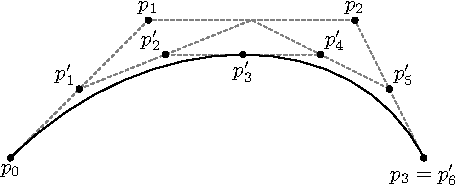
\includegraphics{subdivision}
	     \caption{A Figure}
	 \label{subd}
	\end{figure}

\clearpage %% starts a new page and stops trying to place floats such as tables and figures

\section{More Figure Stuff}
You can also scale and rotate figures.
 	\begin{figure}[h!]
	   
	       \centering
	    % DO NOT ADD A FILENAME EXTENSION TO THE GRAPHIC FILE
	    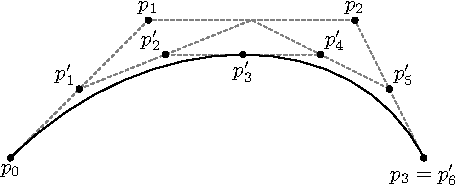
\includegraphics[scale=0.5,angle=180]{subdivision}
	    % if your figure shows up not where you want it, it may just be too big to fit. You can use the scale argument to shrink it, e.g. scale=0.85 is 85 percent of the original size. 
	     \caption{A Smaller Figure, Flipped Upside Down}
	 \label{subd2}
	\end{figure}

\section{Even More Figure Stuff}
With some clever work you can crop a figure, which is handy if (for instance) your EPS or PDF is a little graphic on a whole sheet of paper. The viewport arguments are the lower-left and upper-right coordinates for the area you want to crop.

 	\begin{figure}[h!]
	    	       \centering
	    % DO NOT ADD A FILENAME EXTENSION TO THE GRAPHIC FILE
	   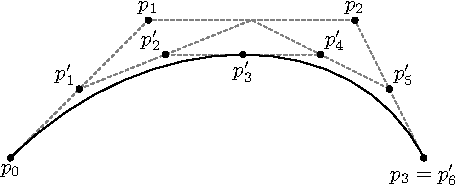
\includegraphics[clip=true, viewport=.0in .0in 1in 1in]{subdivision}
	    \caption{A Cropped Figure}
	 \label{subd3}
	\end{figure}
	
      \subsection{Common Modifications}
      The following figure features the more popular changes thesis students want to their figures. This information is also on the web at \url{web.reed.edu/cis/help/latex/graphics.html}.
    %\renewcommand{\thefigure}{0.\arabic{figure}} 	% Renumbers the figure to the type 0.x
    %\addtocounter{figure}{4} 						% starts the figure numbering at 4
    \begin{figure}[htbp]
    \begin{center}
   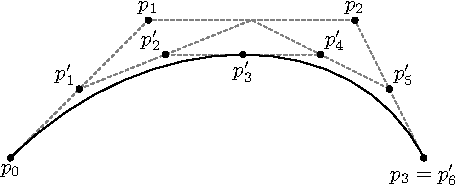
\includegraphics[scale=0.5]{subdivision}
    \caption[Subdivision of arc segments]{\footnotesize{Subdivision of arc segments. You can see that $ p_3 = p_6^\prime$.}} %the special ToC caption is in square brackets. The \footnotesize makes the figure caption smaller
    \label{barplot}
    \end{center}
    \end{figure} 

\chapter*{Conclusion}
         \addcontentsline{toc}{chapter}{Conclusion}
	\chaptermark{Conclusion}
	\markboth{Conclusion}{Conclusion}
	\setcounter{chapter}{4}
	\setcounter{section}{0}
	
Here's a conclusion, demonstrating the use of all that manual incrementing and table of contents adding that has to happen if you use the starred form of the chapter command. The deal is, the chapter command in \LaTeX\ does a lot of things: it increments the chapter counter, it resets the section counter to zero, it puts the name of the chapter into the table of contents and the running headers, and probably some other stuff. 

So, if you remove all that stuff because you don't like it to say ``Chapter 4: Conclusion'', then you have to manually add all the things \LaTeX\ would normally do for you. Maybe someday we'll write a new chapter macro that doesn't add ``Chapter X'' to the beginning of every chapter title.

\section{More info}
And here's some other random info: the first paragraph after a chapter title or section head \emph{shouldn't be} indented, because indents are to tell the reader that you're starting a new paragraph. Since that's obvious after a chapter or section title, proper typesetting doesn't add an indent there. 


%If you feel it necessary to include an appendix, it goes here.
    \appendix
      \chapter{The First Appendix}
      \chapter{The Second Appendix, for Fun}


%This is where endnotes are supposed to go, if you have them.
%I have no idea how endnotes work with LaTeX.

  \backmatter % backmatter makes the index and bibliography appear properly in the t.o.c...

% if you're using bibtex, the next line forces every entry in the bibtex file to be included
% in your bibliography, regardless of whether or not you've cited it in the thesis.
    \nocite{*}

% Rename my bibliography to be called "Works Cited" and not "References" or ``Bibliography''
% \renewcommand{\bibname}{Works Cited}

%    \bibliographystyle{bsts/mla-good} % there are a variety of styles available; 
%  \bibliographystyle{plainnat}
% replace ``plainnat'' with the style of choice. You can refer to files in the bsts or APA 
% subfolder, e.g. 
 \bibliographystyle{APA/apa-good}  % or
 \bibliography{thesis}
 % Comment the above two lines and uncomment the next line to use biblatex-chicago.
 %\printbibliography[heading=bibintoc]

% Finally, an index would go here... but it is also optional.
\end{document}
